% -*- Mode:TeX -*-

%% IMPORTANT: The official thesis specifications are available at:
%%            http://libraries.mit.edu/archives/thesis-specs/
%%
%%            Please verify your thesis' formatting and copyright
%%            assignment before submission.  If you notice any
%%            discrepancies between these templates and the 
%%            MIT Libraries' specs, please let us know
%%            by e-mailing thesis@mit.edu

%% The documentclass options along with the pagestyle can be used to generate
%% a technical report, a draft copy, or a regular thesis.  You may need to
%% re-specify the pagestyle after you \include  cover.tex.  For more
%% information, see the first few lines of mitthesis.cls. 

%\documentclass[12pt,vi,twoside]{mitthesis}
%%
%%  If you want your thesis copyright to you instead of MIT, use the
%%  ``vi'' option, as above.
%%
%\documentclass[12pt,twoside,leftblank]{mitthesis}
%%
%% If you want blank pages before new chapters to be labelled ``This
%% Page Intentionally Left Blank'', use the ``leftblank'' option, as
%% above. 

\documentclass[12pt,twoside]{mitthesis}
\usepackage{lgrind}
%% These have been added at the request of the MIT Libraries, because
%% some PDF conversions mess up the ligatures.  -LB, 1/22/2014
\usepackage{cmap}
\usepackage[T1]{fontenc}
\pagestyle{plain}

%% This bit allows you to either specify only the files which you wish to
%% process, or `all' to process all files which you \include.
%% Krishna Sethuraman (1990).

%\typein [\files]{(chap1, chap2)}
\def\files{all}
\def\all{all}
\ifx\files\all \typeout{Including all files.} \else \typeout{Including only \files.} \includeonly{\files} \fi

\begin{document}

%!TEX root = ./thesis.tex
% -*-latex-*-
% 
% For questions, comments, concerns or complaints:
% thesis@mit.edu
% 
%
% $Log: cover.tex,v $
% Revision 1.8  2008/05/13 15:02:15  jdreed
% Degree month is June, not May.  Added note about prevdegrees.
% Arthur Smith's title updated
%
% Revision 1.7  2001/02/08 18:53:16  boojum
% changed some \newpages to \cleardoublepages
%
% Revision 1.6  1999/10/21 14:49:31  boojum
% changed comment referring to documentstyle
%
% Revision 1.5  1999/10/21 14:39:04  boojum
% *** empty log message ***
%
% Revision 1.4  1997/04/18  17:54:10  othomas
% added page numbers on abstract and cover, and made 1 abstract
% page the default rather than 2.  (anne hunter tells me this
% is the new institute standard.)
%
% Revision 1.4  1997/04/18  17:54:10  othomas
% added page numbers on abstract and cover, and made 1 abstract
% page the default rather than 2.  (anne hunter tells me this
% is the new institute standard.)
%
% Revision 1.3  93/05/17  17:06:29  starflt
% Added acknowledgements section (suggested by tompalka)
% 
% Revision 1.2  92/04/22  13:13:13  epeisach
% Fixes for 1991 course 6 requirements
% Phrase "and to grant others the right to do so" has been added to 
% permission clause
% Second copy of abstract is not counted as separate pages so numbering works
% out
% 
% Revision 1.1  92/04/22  13:08:20  epeisach

% NOTE:
% These templates make an effort to conform to the MIT Thesis specifications,
% however the specifications can change.  We recommend that you verify the
% layout of your title page with your thesis advisor and/or the MIT 
% Libraries before printing your final copy.
\title{Adaptive Consistency Management for Distributed Machine Learning}

\author{Christoph Alt}
% If you wish to list your previous degrees on the cover page, use the 
% previous degrees command:
%       \prevdegrees{A.A., Harvard University (1985)}
% You can use the \\ command to list multiple previous degrees
%       \prevdegrees{B.S., University of California (1978) \\
%                    S.M., Massachusetts Institute of Technology (1981)}
\department{Department of Electrical Engineering and Computer Science}

% If the thesis is for two degrees simultaneously, list them both
% separated by \and like this:
% \degree{Doctor of Philosophy \and Master of Science}
\degree{Master of Science in Computer Science and Engineering}

% As of the 2007-08 academic year, valid degree months are September, 
% February, or June.  The default is June.
\degreemonth{May}
\degreeyear{2017}
\thesisdate{May 11, 2017}

%% By default, the thesis will be copyrighted to MIT.  If you need to copyright
%% the thesis to yourself, just specify the `vi' documentclass option.  If for
%% some reason you want to exactly specify the copyright notice text, you can
%% use the \copyrightnoticetext command.  
%\copyrightnoticetext{\copyright IBM, 1990.  Do not open till Xmas.}
\copyrightnoticetext{}

% If there is more than one supervisor, use the \supervisor command
% once for each.
\supervisor{Prof. Dr. Odej Kao}{Associate Professor}

% This is the department committee chairman, not the thesis committee
% chairman.  You should replace this with your Department's Committee
% Chairman.
\chairman{Prof. Dr. Volker Markl}{Associate Professor}

% Make the titlepage based on the above information.  If you need
% something special and can't use the standard form, you can specify
% the exact text of the titlepage yourself.  Put it in a titlepage
% environment and leave blank lines where you want vertical space.
% The spaces will be adjusted to fill the entire page.  The dotted
% lines for the signatures are made with the \signature command.
\maketitle

% The abstractpage environment sets up everything on the page except
% the text itself.  The title and other header material are put at the
% top of the page, and the supervisors are listed at the bottom.  A
% new page is begun both before and after.  Of course, an abstract may
% be more than one page itself.  If you need more control over the
% format of the page, you can use the abstract environment, which puts
% the word "Abstract" at the beginning and single spaces its text.

%% You can either \input (*not* \include) your abstract file, or you can put
%% the text of the abstract directly between the \begin{abstractpage} and
%% \end{abstractpage} commands.

% First copy: start a new page, and save the page number.
\cleardoublepage
% Uncomment the next line if you do NOT want a page number on your
% abstract and acknowledgments pages.
\pagestyle{empty}
%\setcounter{savepage}{\thepage}
\begin{abstractpage}
%!TEX root = ./thesis.tex
% $Log: abstract.tex,v $
% Revision 1.1  93/05/14  14:56:25  starflt
% Initial revision
% 
% Revision 1.1  90/05/04  10:41:01  lwvanels
% Initial revision
% 
%
%% The text of your abstract and nothing else (other than comments) goes here.
%% It will be single-spaced and the rest of the text that is supposed to go on
%% the abstract page will be generated by the abstractpage environment.  This
%% file should be \input (not \include 'd) from cover.tex.
In recent years, machine learning emerged as the core of many successful applications and businesses.
While the rise of artificial intelligence continues, the amount of data to be processed grows even faster.
Unsurprisingly a lot of research has since focused on methods to parallelize commonly used algorithms and new systems and frameworks have been published, trying to improve the performance of distributed machine learning.
Even though there has been a lot of progress towards more efficient systems, many state-of-the-art systems still have limitations.
Current frameworks are neither expressible nor flexible enough to allow for efficient development of distributed machine learning algorithms, making them unsuited for experimentation and quick prototyping even though this is essential for achieving optimimal performance.
On the other hand, most parallelization strategies exploit the algorithms inherent stochastic nature to enable parallel execution at the expense of lowered consistency among the shared state.
Even though this does not necessarily affect quality of the results, an improper choosen level of consistency can severely affect algorithm performance, resulting in a non optimal convergence rate and therefore increased runtime.

This thesis introduces a novel framework for distributed machine learning, which is based on a state centric programming model with yield semantics.
The programming model allows the user to focus on the key elements of developing distributed machine learning algorithms, namely parameter communication, parameter merging and adaptive consistency management among distributed workers, while the system takes care of utilizing the cluster resources in an optimal fashion.
The experiments using elastic-net regularized linear regression show an increased performance compared to state-of-the-art data processing systems like Apache Spark and at the same time reduce the effort of developing, parallelizing and experimenting with distributed machine learning algorithms at scale.

\end{abstractpage}

% Additional copy: start a new page, and reset the page number.  This way,
% the second copy of the abstract is not counted as separate pages.
% Uncomment the next 6 lines if you need two copies of the abstract
% page.
\setcounter{page}{\thesavepage}
%\begin{abstractpage}
%!TEX root = ./thesis.tex
% $Log: abstract.tex,v $
% Revision 1.1  93/05/14  14:56:25  starflt
% Initial revision
% 
% Revision 1.1  90/05/04  10:41:01  lwvanels
% Initial revision
% 
%
%% The text of your abstract and nothing else (other than comments) goes here.
%% It will be single-spaced and the rest of the text that is supposed to go on
%% the abstract page will be generated by the abstractpage environment.  This
%% file should be \input (not \include 'd) from cover.tex.

%\end{abstractpage}

\cleardoublepage

\section*{Acknowledgments}

First and foremost, I would like to thank Prof. Dr. Odej Kao and Prof. Dr. Volker Markl for supervising my thesis and the opportunity to write this thesis in cooperation with the Department of Complex and Distributed IT Systems.
I would also like to thank Tobias Herb for his supervision, guidance and highly valuable input.
This thesis would not have been possible without his excellent work on the framework.
I would like to thank Morgan Geldenhuys and Daniel Schr\"oder for the countless hours of inspiring discussions.
I am very thankful to my girlfriend Anja who has been with me, encouraging me and providing me with support to finally complete this journey.
Last but not least, I would like to thank my parents for their never ending support.

%%%%%%%%%%%%%%%%%%%%%%%%%%%%%%%%%%%%%%%%%%%%%%%%%%%%%%%%%%%%%%%%%%%%%%
% -*-latex-*-

% Some departments (e.g. 5) require an additional signature page.  See
% signature.tex for more information and uncomment the following line if
% applicable.
 %Eidesstattliche Erklärung
Hiermit erkläre ich Eides statt, dass ich dir vorliegende Arbeit selbstständig und ohne unerlaubte fremde Hilfe angefertigt, andere als die angegebenen Quellen und Hilfsmittel nicht benutzt und die den benutzten Quellen wörtlich oder inhaltlich entnommenen Stellen als solche kenntlich gemacht habe.


Unterschrift Ort, Datum

\pagestyle{plain}
% -*- Mode:TeX -*-
%% This file simply contains the commands that actually generate the table of
%% contents and lists of figures and tables.  You can omit any or all of
%% these files by simply taking out the appropriate command.  For more
%% information on these files, see appendix C.3.3 of the LaTeX manual. 
\tableofcontents
\newpage
\listoffigures
\newpage
%\listoftables

\chapter{Introduction}
One of the most challenging tasks in computer science and engineering resolves around improving algorithm performance.
In general this has been done by making hardware faster and inventing new strategies and algorithms to parallelize work more efficiently.
Since it is clear that Moore's Law will not hold anymore, a lot of effort has been spent to horizontally scale algorithm computation across multiple machines.
Machine learning is no exception and efficient parallelization is a key aspect towards more intelligent systems.
By now, many general purpose frameworks for large scale data processing have been developed and published. Many of those are used for running more complex machine learning algorithms at scale as well.
Unfortunatelly, the performance often is not satisfying due to the architecture and programming model not reflecting the underlying structure of most commonly used machine learning algorithms.
Common data processing tasks can be represented as an extract-transform-load (ETL) pipeline, which is often easily parallelizable. This does not hold for machine learning, where algorithms are mostly sequential in nature and the only way of achieving parallelism is by exploiting their inherent stochastic properties. This allows to break the sequential execution in favor of parallel learning on subsets, which then needs to be combined in order to obtain a solution to the global task.
While this can lead to a great speedup in terms of processed data, it can have a negative affect on the learning progress.
Therefore a key part of horizontally scaling machine learning algorithms is to ensure all participating learners have a consistent view on each others progress while at the same time maintaining a tradeoff between communicating progress and actually executing the learning task.


\section{MapReduce and Beyond}
Many of todays successful businesses throughout fields like finance, e-commerce and healthcare rely heavily on the ability to process vast amounts of user or sensorical data, collected to make their services smarter and ultimatelly their user experience better.
In order to learn from the collected data, discover patterns and ultimately gain new insights, it needs to be processed by an algorithm.
It is not uncommon that the input ranges somewhere between hundred gigabytes and tenth of petabytes.
In the past, processing this much data required either a supercomputer, which was only available to large institutions or government entities or some proprietary compute cluster.
All this changed when Google introduced MapReduce \cite{Dean2004} in 2004.
The MapReduce framework made it possible to process data in a distributed and fault tolerant way with the help of a compute cluster formed by hundredth or thousandth of machines.
Instead of using a single, expensive, special hardware supercomputer the framework provides the foundation to assemble commodity hardware machines into a compute cluster.
The framework takes care of all necessary aspects to ensure a fault tolerant and parallel execution of a task submitted to the cluster.
The advantage compared to previous approachs is that the framework can be run entirely on top of machines using commodity hardware, which does not require special hardware and therefore equals low cost.

MapReduce esentially led the path to a convenient and widespread use of big data processing, which found its open source implementation in the Apache Hadoop project \cite{hadoop2009hadoop}.
The project quickly gained traction and has spawned many business grade platforms, which quickly gained widespread adoption and by now provides a whole ecosystem around big data processing. The software stack includes a fault tolerant distributed filesystem (HDFS) a MapReduce framework and a cluster resource manager (YARN) \cite{KumarVavilapalli2013}.
On the other hand, MapReduce suffers from some practical limitations that lead to the development of new, more sophisticated and specialised big data frameworks. With the most widely used frameworks being Apache Spark \cite{Zaharia2010}, Apache Flink \cite{Alexandrov2014} and GraphLab \cite{Low2012}.
The first two frameworks use at it's core a dataflow pipeline based architecture, whileas the latter uses a graph abstraction to model particular algorithms.
All this works well for algorithms that can be expressed as an extract-transform-load (ETL) pipeline and are often embarrassingly parallel in nature.
On the other hand, machine learning algorithms often rely heavily on many, computationally light, iterations to iteratively update a shared state (model) such as logistic regression or latent dirichlet allocation (LDA).
These so called iterative-convergent algorithms required a change in how systems for distributed large scale machine learning operate at its core.


\section{Distributed Machine Learning}
This limitation sparked the development of frameworks specialized for distributed execution of iterative-convergent algorithms used in common machine learning tasks.
The most widely recognized systems are Petuum \cite{Xing2015}, ParameterServer \cite{Li2014} and MALT \cite{Li2015}.
Different from the MapReduce paradigm these frameworks, instead of using a pipeline to transform an immutable dataset into another immutable dataset, operate on a fixed but mutable state, which is held by a single machine or distributed over multiple machines.
This state can then be updated by workers that have computed an update locally and send it to these state keepers. Which act as surrogates, taking state updates and incorporating these into the state by some user defined function.
While these systems can increase the performance on machine learning algorithms by an order of magnitude (c) compared to dataflow systems, most systems come with either limited usability, which makes it difficult to implement additional algorithms, are tied to a specific algorithm or are very low level frameworks.
Efficiently distributing machine learning algoritms while at the same time provide the ability to conscisely express machine learning algorithms remains and extremely challenging problem.
A system targeting the execution of those algorithms at scale must therefore provide the ability to conscisely express the underlying algebraic structure and at the same time be flexible enough to allow experimentation and fine tuning.
Where consistency management is an essential part to ensure that algorithms are executed both fast and also learning performance is well enought.


\section{Thesis Outline}
In this thesis we introduce a novel framework for large scale distributed machine learning.
It improves upon currently available systems by providing a powerful programming abstraction that can conscisely express state of the art machine learning algorithms and at the same time minimizes the effort necessary to move from a single machine to a cluster.
The framework design is optimized for efficient parallel execution of iterative-convegent algorithms in a cluster and ensures the required consistency is enforced among parallel learners, depending on the algorithm properties. By maintaining the best tradeoff between algorithm execution and progress communication the performance is improved as well.
All of this can be easily customized for quick prototyping and finetuning, which makes the system suited for developers as well as researchers.
I start off by providing background knowledge on state of the art dataflow systems and their internals in chapter \ref{c:background}, followed by a formal explaination of iterative-convergent algorithms. Both provide the foundation to understand why current dataflow systems are unsuited for many large scale distributed machine learning applications.
I provide an overview over the important parts that need to be considered when developing a distributed machine learning system and how this is achieved by current frameworks.
Chapter \ref{c:state_centric} introduces the state centric programming model, which treats the state as a mutable first class citizen, which can be distributed and alter by updates that result from computation according to the algorithm that is executed.
This allows the system to reason about the most optimal distribution of state in the cluster which is then collocated with computation that can update the state. I further describe the architecture of the system and how the essential components are implemented.
When updating the state from multiple different locations, consistency must be maintained in order to ensure that algorithm progresses as expected, which is the responsibility of the state to manage its consistency among all of its instances in the cluster. I implemented several schemes that target machine learning algorithms and their stochastic properties in order to limit the synchronization required, which decreases the network bandwidth required.
At the end I summarize the experiments with the lessons learned and provide suggestions on how to further improve systems for large scale distributed machine learning.

Improving speed, allowing more degrees of freedom (async program flow), ease the development of algorithms close to single machine implementations, compiler, letting the developer and researcher choose the strategy if necessary or implement heuristics <- challenge and motivation

Background
State Centric Programming Model
Consistency Management
Experiments
Wrap Up
%!TEX root = ./../thesis.tex

\chapter{Background}
\label{c:background}
This section provides the necessary background to follow the argumentation in the following chapters regarding state centric programming model and consistency management.
This includes an understanding of algorithms and optimization techniques commonly used in practice (not limited to distributed machine learning), the current state-of-the-art in dataflow systems and how dataflow is used to provide a fault tolerant and distributed framework for large scale data processing and machine learning.
Furthermore the field of distributed machine learning is explained in more detail, including the current state-of-the-art frameworks used for this purpose, their limitations and challenges that arise when machine learning algorithms are parallelized in a distributed fashion among multiple physical machines.


\section{Algorithms and Optimization}

\subsection{Iterative Convergent Algorithms}
\label{ss:ica}
Consider a supervised learning setup with a dataset $D = \{z_1,\ldots,z_n\}$ with each example $z_i$ being represented by a pair $(x_i,y_i)$ consisting of an input $x_i$ and a scalar output $y_i$.
Consider also a loss function $\ell(\hat{y},y)$ quantifying the cost of predicting $\hat{y}$ when the true output is $y$. As a model, a family $F$ of functions $f_w(x)$ parameterized by a weight vector $w$ is chosen.
The goal is to find a function $f \in F$ that minimizes the loss $Q(z, w) = \ell(f_w(x),y)$. Emperical risk $E_n(f) = \frac{1}{n}\sum_{i=0}^{n}\ell(f(x_i),y_i)$ performance on training set, expected risk generalization performance.
\begin{equation}
E_n(f_w) = \frac{1}{n}\sum_{i=0}^{n} \ell(f_w(x_i),y_i)
\label{eqn:emp_risk}
\end{equation}
In order to find an optimal solution many algorithms used in large scale machine learning such as regression, topic models, matrix factorization or neural networks employ either gradient based methods or markov chain monte carlo methods.
To obtain the optimal solution those algorithms try to iteratively update the weight vector $w$. At each iteration $t$ an updated weight vector $w^{t}$ is computed based on the vector of the previous iteration $w^{(t-1)}$ and the data $D$. The resulting model $f_{w^{t}}$ is again a better summary of the data $D$ under the objective $Q$. \ref{eqn:delta_upd} shows the process of refining the model, with $\Delta$ being an arbitrary update function.
\begin{equation}
w^{t} = w^{(t-1)} + \Delta(w^{(t-1)},D)
\label{eqn:delta_upd}
\end{equation}
The update function depends on the algorithm employed and can be viewed as a procedure of obtaining a step towards a better model. At each iteration an update $\Delta w$ is computed and applied to the previous weight vector until a stopping condition is satisfied. E.g. the distance to the optimal solution or the objective difference between two iterations is monitored. When the difference is below a certain threshold the computation stops and the algorithm is said to be converged.


\subsection{Convex Optimization}
\label{ss:optimization}
In order to estimate the optimal parameters $w^*$ of a function belonging to class $f_{w^*} \in F$, numerous techniques can be employed to estimate said parameters.
In many cases, especially large scale machine learning methods such as (stochastic) gradient descent and coordinate ascent are used to iteratively optimized the parameterization of the chosen function class.
Both techniques represent different rules of computing the update shown in \ref{eqn:delta_upd}.
Gradient descent updates the weights $w$ at each iteration $t$ on the basis of the gradient of $E_n(f_w)$,
\begin{equation}
w^{t} = w^{(t-1)} - \eta\frac{1}{n}\sum_{i=0}^{n}\nabla_wQ(z_i,w^{(t-1)})
\label{eqn:gd_update}
\end{equation}
where $\eta$ is a chosen gain, often refered to as learning rate.
While this achieves linear convergence under sufficient regularity assumptions and a sufficiently small learning rate $\eta$ \cite{dennis1996numerical} \cite{bottou2010large} a more simplified version is commonly used in practice, called stochastic gradient descent (SGD).
Instead of computing the gradient $\nabla_wE_n(f_w)$ exactly, the gradient is estimated at each iteration $t$ based on a single randomly picked example $z_t$.
\begin{equation}
w^{t} = w^{(t-1)} - \eta_t\nabla_wQ(z_t,w^{(t-1)})
\label{eqn:sgd_update}
\end{equation}
The assumption is that the gradient obtained by \ref{eqn:sgd_update} behaves similar to its expectiation in \ref{eqn:gd_update}.
The convergence properties have been studied extensively and under mild conditions an almost sure convergence can be established when the learning rate satisfies the conditions $\sum_t\eta_t^2 < \infty$ and $\sum_t\eta_t = \infty$ \cite{bottou2010large}.
The general structure of stochastic gradient descent is described in Algorithm \ref{alg:sgd}.

\begin{algorithm}
\caption{Stochastic Gradient Descent}\label{alg:sgd}
\begin{algorithmic}[1]
\State $k\gets 1$ and initialize $w^0 \in \mathbb{R}^d$
\Repeat
\For{}
\State $w^{t} \gets w^{(t-1)} - \eta_t\nabla_wQ(z_t,w^{(t-1)})$
\EndFor
\Until{termination criteria satisfied}
\end{algorithmic}
\end{algorithm}

Coordinate descent on the other hand iteratively tries to optimize a given objective by successively performing approximate minimization along a coordinate direction while keeping the other directions fixed.
TODO: give a more in detail explanation and provide algorithm description

\begin{algorithm}
\caption{Stochastic Coordinate Ascent}\label{alg:sca}
\begin{algorithmic}[1]
\State $k\gets 1$ and initialize $w^0 \in \mathbb{R}^d$
\Repeat
\For{}
\State
\EndFor
\Until{termination criteria satisfied}
\end{algorithmic}
\end{algorithm}

\subsection{Regularization}

\begin{equation}
Q(z,w) = \textit{$\ell$}(f_w(x),y) + \textit{r}(w)
\label{eqn:l1_reg}
\end{equation}

\begin{equation}
Q(z,w) = \textit{$\ell$}(f_w(x),y) + \textit{r}(w)
\label{eqn:l2_reg}
\end{equation}

\begin{equation}
Q(z,w) = \textit{$\ell$}(f_w(x),y) + \textit{r}(w)
\label{eqn:elastic_net}
\end{equation}

NOTES:
- regularization in general
- L1, L2 regularization
- elastic-net as special case
- convexity properties
- mini-batch setup algorithm


\subsection{CoCoA}
Due to their widespread application in large scale machine learning and recent advances in the field of distributed optimization the thesis focuses on linear regularized objectives.
The theroretical contemplation as well as the experiments in Section \ref{c:experiments} focus on a framework for convex optimization problems called CoCoA (Communication-efficient distributed dual Coordinate Ascent) \cite{Jaggi2014} and its successors CoCoA$^+$\cite{smith2015l1} and PROXCoCoA$^+$\cite{smith2016cocoa}.
CoCoA as described in Algorithm \ref{alg:cocoa} provides a communication-efficient framework for solving convex optimization problems of the following form
\begin{equation}
\min_{\alpha} Q(z,\alpha) = \ell(f_\alpha(x),y) + r(\alpha)
\label{eqn:lin_loss}
\end{equation}
in a distributed setting.
Where $\alpha$ denotes the weight vector, $\ell$ is convex and smooth and $r$ is assumed to be seperable, which in this context means $r(x) = \sum_{i=0}^nr_i(x_i)$.
Commonly the term $\ell$ is an emperical loss over the data of the form $\sum_{i} \ell(f_w(x_i), y_i)$ and the term $r$ is a regularizer, e.g. $r(w) = \lambda\|w\|_p$ where $\lambda$ is a regularization parameter.
Many algorithms in machine learning can be expressed in this form, such as logistic and linear regression, lasso and sparse logistic regression and support vector machines.

CoCoA leverages the primal-dual relation which allows for solving the problem in either the primal or dual formulation.
For some application where the number of examples $n$ is much smaller than the number of features $d$, $n way lesser than d$, solving the problem in the dual may be easier because this problem has $n$ variables to optimize, compared to $d$ for the primal.
The CoCoA framework leverages Fenchel-Rockafellar duality to quadratically approximate the global objective in \ref{eqn:lin_loss}.
This leads to separability of the problem over the coordinates of $\alpha$ and the partitions, where the local subproblems are similar in structure to the global problem and also exploit second order information within the local data partition.
Therefore the dataset $D \in \mathbb{R}^{d \times n}$ can be distributed either example-wise or feature-wise over $K$ physical machines according to the partitioning $\{P\}_{k=1}^K$, depending which is more efficient to solve.
The size of the partition on machine $k$ is denoted by $n_k = \mid P_k \mid$.
The key to efficient distributed optimization is that the local subproblems can be solved independently on each worker in parallel and only a single parameter vector $v = \nabla f(D\alpha) \in \mathbb{R}^n$ needs to be shared after each round in order to communicate the progress of each local worker on its subproblem.
As the data stays local and only a single parameter vector of dimension $n$ needs to be exchanged, CoCoA is very communication efficient and as the local subproblems are very similar to the global problem, arbitrary solvers can be employed as well.
The local quadratic subproblem has the following form
\begin{equation}
\min_{\alpha_{[k]} \in \mathbb{R}^n} \zeta_k^{\sigma^\prime}(\Delta\alpha_{[k]}, v, \alpha_{[k]}),
\label{eqn:min_local_subp}
\end{equation}
where
\begin{equation}
\zeta_k^{\sigma^\prime}(\Delta\alpha_{[k]}, v, \alpha_{[k]}) = \frac{1}{K}f(v) + w^TA_{[k]}\Delta\alpha_{[k]} + \frac{\sigma^\prime}{2\tau}\|A_{[k]}\Delta\alpha_{[k]}\|^2 + \sum_{i \in P_k}g_i(\alpha_i + \Delta\alpha_{[k]_i}),
\label{eqn:local_subp}
\end{equation}
with $A_{[k]}$ refering to the the local data and $w = \nabla f(D\alpha) \in \mathbb{R}^n$.
$\alpha_{[k]_i}$ denotes the local weight vector stored on machine $k$ with $\alpha_{[k]_i} = \alpha_i$ if $i \in P_k$ otherwise $\alpha_{[k]_i} = 0$.
\begin{algorithm}
\caption{CoCoA Framework}\label{alg:cocoa}
\begin{algorithmic}[1]{}
\DATA Data matrix $D$, distributed column-wise according to partition $\{P_k\}_{k=1}^K$
\INPUT aggregation parameter $\gamma \in (0,1]$, subproblem parameter $\sigma^\prime$
\INIT $t \gets 0$, $\alpha^{(0)} \gets 0 \in \mathbb{R}^n$, $v^{(0)} \gets 0 \in \mathbb{R}^d$ 
\Repeat
\State $t \gets t + 1$
\For{$k \in \{1,\ldots,K\}$}
\State obtain an approximate solution $\Delta\alpha_{[k]}$ for the local subproblem \ref{eqn:min_local_subp}
\State update local weights $\alpha_{[k]}^{t} = \alpha_{[k]}^{t-1} + \gamma\Delta\alpha_{[k]}$
\State update shared parameter vector $\Delta v_k = A_{[k]}\Delta\alpha_{[k]}$
\EndFor
\State compute $v^{t} = v^{t-1} + \gamma\sum_{k=1}^K\Delta v_k$
\Until{termination criteria satisfied}
\end{algorithmic}
\end{algorithm}
In summary the framework provides a procedure to effectively combine the results from local computation without having to deal with conflicts resulting from similar updates computed on other machines.

NOTES:
- local solver (batch coordinate descent)
- elastic-net in the cocoa setup
- algorithm parameters sigma and gamma


\section{Dataflow Systems}
\label{s:dataflow}
NOTES:
- description of dataflow in general
- architecture of dataflow systems, Apache Spark and Flink
- description of RDDs

\section{The Challenges of Distributed Machine Learning}
\label{s:distributed_ml}
While the execution of iterative-convergent algorithms on a single machine is straightforward, time constraints and the ever growing amount of data to be processed require these algorithms to be executed in parallel.
This posses a number of challenges which are often observed when parallelizing algorithms, such as partitioning the state used in the algorithm as well as communication and consistency management.
In this context, state refers to a structure containing arbitrary data e.g. an array, tensor or list.
While intra-node parallelism in multi-core and multi-processor systems can mitigate these problems, it is not satisfying in terms of cost and scalability.
On the other hand, inter-node parallelism has the desired properties but can not be easily parallelized.
Therefore in the past decade a lot of research has focused on inventing new systems to deal with those challenges and make distributed machine learning more efficient and scalable.

\subsection{State Partitioning}
Depending on the algorithm and optimization technique employed to solve for the optimal solution, there exist multiple approches to distribute the state used in the algorithm (e.g. input data, model parameters).
As depicted in Figure \ref{fig:data_parallelism}, an initial approach by Zinkevich et. al \cite{zinkevich2010parallelized} introduced a data-parallel approach for computing stochastic gradient descent (SGD) via the MapReduce framework.
\begin{figure}[ht]
\centering
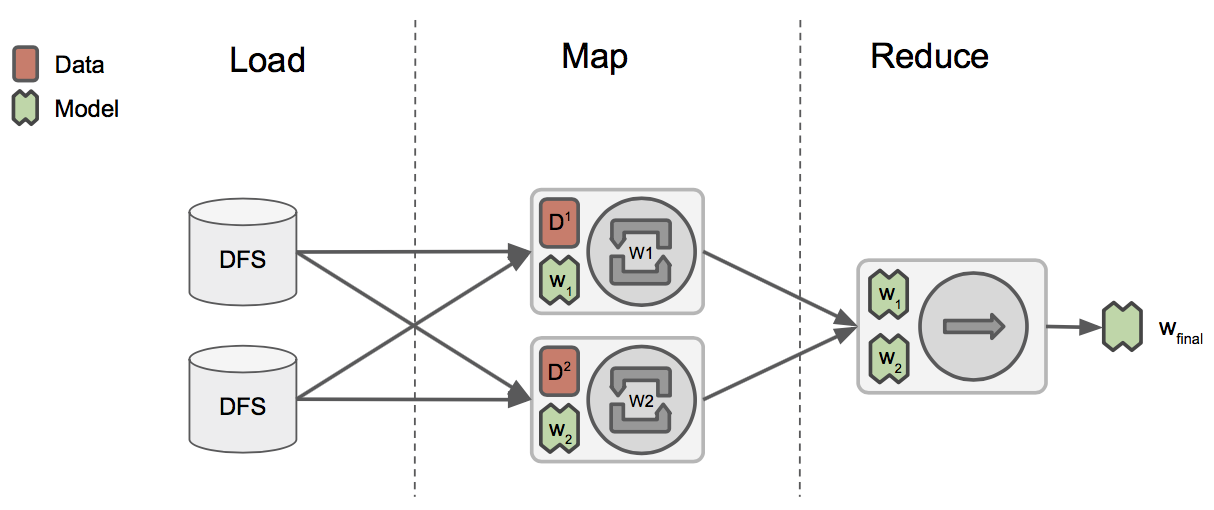
\includegraphics[width=0.9\textwidth]{img/data_parallelism.png}
\caption{Data-parallelism via MapReduce}
\label{fig:data_parallelism}
\end{figure}
In this context, data-parallelism means that $K$ machines work in parallel on the input data $D$, hence the data is distributed according to partition $\{P_k\}_{k=1}^K$ into local parts $D^k$.
Each machine maintains a local model $w_k$ that is iteratively refined based on \ref{eqn:delta_upd} until convergence, using only the local part of the input data $D^k$.
The local update is of the form
\begin{equation}
w_k^{t} = w_k^{t-1} + \Delta(w_k^{t-1},D^k)
\label{eqn:local_delta_upd}
\end{equation}
The final model $w_{final}$ is then obtained in the reduce step by averaging over all local models $w_{k}$.
\begin{equation}
w_{final} = \frac{1}{K}\sum_{k=1}^{K}w_{k}
\label{eqn:avg_sgd}
\end{equation}
Even though this approach works well in practice and gives considerable good results, it suffers from two limitations.
First, if the size of a local model $w_k$ exceeds the available memory on a single machine, the algorithm can not work properly.
This is the case e.g. for topic models at web scale or deep neural networks used in the Google Brain project \cite{dean2012large}, consisting of billions of parameters.
Second, even though the scalability improved by introducing data-parallelism the lack of parameter exchange during runtime can lead to suboptimal performance \cite{xing2015strategies} as the algorithm essentially resembles batch gradient descent, which is known to have suboptimal convergence properties compared to mini-batch or stochastic gradient descent \cite{bottou2010large} \cite{smith2016cocoa}.
In order to improve the performance, a system must be able to communicate more frequently and it must also be able to partition a model accross multiple machines to scale with the size of the model.
Following those requirements resulted in the publication of the parameter server \cite{Li2014}, which provides a framework for inter-node parallelism of iterative convergent algorithms.

\subsection{Communication}
As depicted in Figure \ref{fig:param_server}, the parameter server is a group of an arbitrary number of machines $\{S\}_{l=1}^L$, e.g. $S = \{S_1, S_2\}$ where each member of the group is responsible for storing a part of the model $\{w\}_{l=1}^L$ and making it accessible to the workers $\{W\}_{k=1}^K$, e.g. $W = \{W_1, W_2, W_3\}$, via a defined interface that is similar to a key-value store.
The model is partitioned among the machines of the server to provide optimal throughput, fault tolerance and to mitigate the effect of a model exceding the memory of a single machine.
\begin{figure}[ht]
\centering
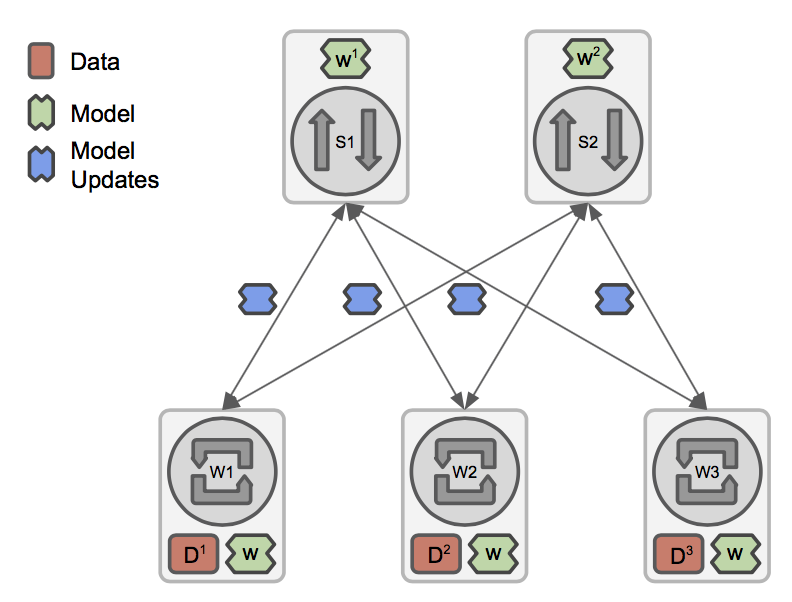
\includegraphics[width=0.7\textwidth]{img/param_server.png}
\caption{Parameter Server}
\label{fig:param_server}
\end{figure}
Each of the workers maintains a local partition of the input data $\{D\}_{k=1}^K$, which is used to iteratively compute updates for the parameters $w$ according to
\begin{equation}
\Delta w_{k_i}^{t} = \Delta(w_{k_i}^{t-1},D^k).
\label{eqn:local_delta_upd_param}
\end{equation}
In the parameter server setup, the local state $w$ acts as a cache for global parameters in order to reduce network usage.
Therefore, depending on the caching policy, $w_{k_i}$ can either be directly read either the local cache or must be retrieved from the parameter server.
Additionally to applying the update to the local model $w$, the difference $\Delta w_{k_i}^{t}$ is published to the parameter server as well, which takes care of applying it to the corresponding entry $w_i$ to make the update available to all other workers $W_i$, $i \neq k$.
In case multiple updates for the same parameter $w_i$ arive at the same time, a user defined function (UDF) needs to be provided to the server, which takes care of combining those updates so it can be applied to the parameter stored on the server.
The procedure of retrieving, updating and publishing is executed concurrently on all workers.
This enables all workers to work in parallel on the iterative parameter refinement while asynchronously updating and retrieving the parameters necessary for computing the next update.
The procedure of updating the model in parallel is also known as model-parallelism.

While this schema has been proven to work well in practice (some numbers), a couple of issues still remain when running iterative-convergent algorithms at scale using the parameter server.
According to \cite{wei2015managed} this can be viewed as finding the trade-off between algorithm throughput and data throughput.
In other words the challenge is to find a balance between the quality of parameter refinements and the quantity at which they are generated.
As with distributed systems in general, network commmunication is the bottleneck in distributed machine learning as well.
Even though due to the stochastic nature of many machine learning algorithms, the communication can be reduce compared to the exact serial algorithm, it has been proven that fresher model parameters increase the algorithm throughput per iteration \cite{langford2009slow}.
Therefore, in order to guarantee an optimal algorithm throughput, a worker should always work with the latest parameters.
On the other hand, exchanging parameter updates over the network more frequently is time consuming, which leaves less time to run local computation and therefore essentially decreases the data throughput due to increased time spent on network management.
The second issue concerns the relaxed consistency among participating workers due to reduced communication compared to the serial algorithm.
Though this is what makes the parameter server concept so powerful because it increases the data throughput by relaxing the consistency requirements when updating parameters on the server.
By decoupling the progress of workers it is possible to minimize the effect of stragglers and synchronization delay between workers \cite{ananthanarayanan2013effective}.
However, as discussed in the next section, combining model parameters obtained from workers with greatly differing algorithm progress can have a detrimental effect on algorithm throughput.
Finding the balance between algorithm throughput and data throughput can therefore be seen as consistency management.


\subsection{Consistency}
The most important part of any distributed system is the synchronization strategy used to ensure consistency among multiple machines concurrently accessing and updating some shared state.
In distributed machine learning the shared state is the model, which is for example stored in a parameter server and continously refined by updates locally computed by a worker and then published to the server.
There are three schemes used to synchronize workers during the iterative parameter refinement.
\textit{Bulk synchronous parallelization (BSP)} leads to the best algorithm throughput (convergence achieved per number of examples processed).
In this scheme, all workers are required to finish their current iteration and at the end successfully publish all updates to the parameter server.
The server then computes a refined model $w^t$ according to \ref{eqn:bsp_upd} and each worker retrieves the updated parameters before beginning the next iteration.
This synchronization scheme guarantees consistency among all nodes at all times.
\begin{equation}
w^{t} = w^{t-1} + \frac{1}{K}\sum_{k=1}^{K}\Delta(w^{t-1}_{k}, D{k})
\label{eqn:bsp_upd}
\end{equation}
While this synchronization strategy essentially recovers the sequential algorithm for a single machine and has the same convergence properties and guarantees, it suffers from a severe limitation when used in a distributed setup \cite{langford2009slow}.
In case one of the workers is for some reason a lot slower than the others the synchronization barrier imposed by BSP forces all workers to wait for this particular worker in the group.
This is well known as the straggler problem \cite{ananthanarayanan2013effective} and can seriously affect performance in a distributed environment, because the progress is limited by the slowest node in the cluster.
BSP is commonly used in MapReduce frameworks such as Hadoop and data-flow systems like Apache Spark and Apache Flink to ensure correct program execution.
The second strategy is known as \textit{total asynchronous parallelization (TAP)}.
Similar to BSP, all workers publish their locally computed parameter updates to the server after each iteration but in this case the changes are applied to the model immediately.
Therefore no waiting for other workers is required, resulting in a very high data throughput.
The straggler problem can be mitigated by this synchronization scheme as well, as depicted in Figure \ref{fig:tap_straggler}.
\begin{figure}[ht]
\centering
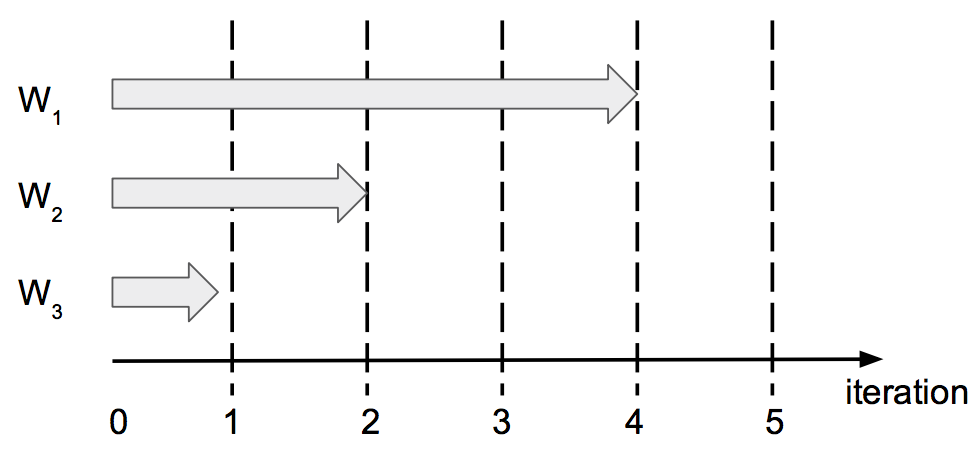
\includegraphics[width=0.6\textwidth]{img/tap_straggler.png}
\caption{Straggler in TAP}
\label{fig:tap_straggler}
\end{figure}
Even though worker $W_3$ is a straggler, which would have prevented the remaining workers $\{W_2, W_3\}$ from proceeding beyond the synchronization barrier of iteration 1, the workers can continue with their next iterations without waiting for the slower worker.
Although this consistency scheme seems to work quite well in practice \cite{Li2014}, it lacks formal convergence guarantees and can even diverge \cite{dai2014high}.
This stems from the fact that no theoretical convergence bound can be established as the divergence in iteration between workers is unbound.
\begin{figure}[ht]
\centering
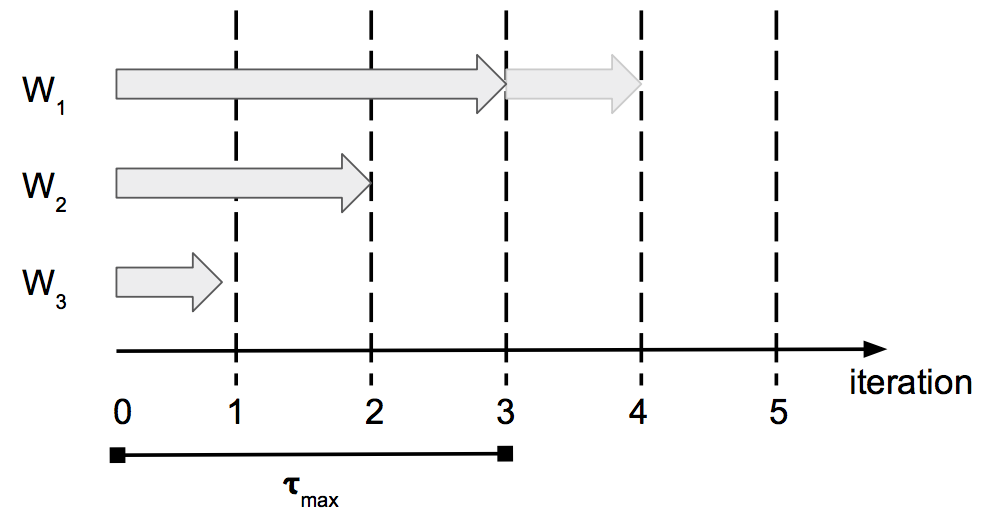
\includegraphics[width=0.6\textwidth]{img/ssp_straggler.png}
\caption{Straggler in SSP}
\label{fig:ssp_straggler}
\end{figure}
A middle ground between bulk synchronous parallelization and total asynchronous parallelization is \textit{stale synchronous parallel (SSP)} \cite{ho2013more} or \textit{bounded staleness (BS)}.
As shown in Figure \ref{fig:tap_straggler}, SSP introduces a fixed maximum delay, or staleness threshold, of $\tau_{max}$ between the slowest and fastest node.
In the example, for $\tau_{max} = 3$ worker $W_1$ is blocked and can not proceed beyond iteration 3 as the slowest worker $W_3$ has not finished its first iteration.
As soon as worker $W_3$ has completed its first iteration, $W_1$ is unblocked and can proceed as long as the difference in iteration stays below $\tau_{max}$.
SSP overcomes some of the limitations of TAP by introducing a bound on divergence in number of iterations between workers.
The staleness threshold resembles a bound which can be used to restore formal convergence guarantees while still maintaining the flexibility of asynchronous parallelization and limiting but not completely preventing the straggler problem \cite{cipar2013solving}.
In general this helps to compensate e.g. update related communication between iterations or fluctuations in worker performance, which explains why SSP works so well in practice.

\chapter{State Centric Programming Model}
\label{c:state_centric}

%!TEX root = ./../thesis.tex

\chapter{Consistency Management}
\label{c:consistency_mgmt}
Consistency management in the context of distributed machine learning describes the process of ensuring an algorithm is parallelized most efficiently without loosing its correctness.
Iterative-convergent algorithms are mostly sequential in nature and parallelization is commonly achieved by exploiting their inherent stochastic properties \cite{herb2016weak}.
Staying with the example of the previous section, as shown in Figure \ref{fig:ica_control_flow}, unit $\Omega_2$ of training step (C) is parallelized with a dop of $K = 2$ by partitioning the input data $D$ and replicating the model $w$ across all parallel units $\{\Omega_{2j}\}_{j=0}^K$.
Proper consistency management targets two domains of the algorithm execution process.
First, as discussed in Section \ref{ss:synchronization}, the control-flow must be synchronized properly according to the transformation applied during the execution of a unit $\Omega_i$ and its replicas $\{\Omega_{ij}\}_{j=0}^K$.
In the example, the loop in (B) and its containing units $\Omega_{2j}$ are defined as SSP in order to increase the data throughput on the input data $D$.
Ultimately this is supposed to result in a better overall performance due to a lower dependency on other units.
Unfortunately, increasing the data throughput alone does not necessarily lead to a better overall performance, as each unit $\Omega_{2j}$ now works independently on a replica $w_j$ of the model without sharing the local progress.
As discussed in Section \ref{ss:consistency}, this staleness of state has a negative effect on the algorithm throughput and can be mitigated by frequently exchanging the updates applied to a state, in this case $w$, between all units $\Omega_{2j}$.
Exchanging updates on the other hand has a negative effect on the data throughput as more computation time must be spent on network management.
Adaptive consistency management therefore is responsible for controlling the best trade-off between communication and computation, based on the requirements for synchronization and consistency at each step of the algorithm as well as continuous feedback about cluster metrics and algorithm progress.

\section{Adaptive Consistency Management}
Consistency management in general can be seen as a cooperative task between the driver and the machines involved in executing the workload defined by the algorithm definition.
Figure \ref{fig:adapt_consist_mgmt} depicts the architecture and connections between driver and machines, where the interpreter is responsible for instructing the machines according to the given program flow and also taking care of managing unit and state life cycles.
\begin{figure}[ht]
\centering
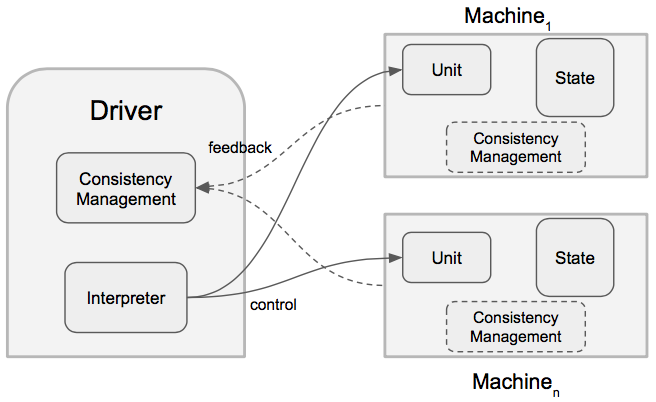
\includegraphics[width=0.7\textwidth]{img/adapt_consist_mgmt.png}
\caption{Adaptive Consistency Management Architecture}
\label{fig:adapt_consist_mgmt}
\end{figure}
The first part of the consistency management resides on the driver and is responsible for collecting feedback from the machines.
This is then used to exercise further control over the algorithm execution.
Feedback can be metrics about the machines, such as resource usage, network bandwidth consumption or algorithm specific properties such as the convergence rate.
Based on the collected feedback, the consistency management is able to provide instructions for the interpreter in order to influence the consistency on a unit level such as the synchronization between parallel instances of a unit in order to improve the algorithm throughput.
Furthermore, the second part of the consistency management resides on each machine.
This is necessary to gain control over the state level consistency as discussed in the previous section.
Consistency management on a state level becomes necessary when a unit is parallelized by creating replicas on multiple machines.
Parallelizing a unit results in replication or partitioning of the attached states and therefore it is necessary to control the communication frequency of model or parameter updates based on the available network bandwidth or some network quota.
Also it is in general possible to control algorithm specific parameters such as the learning rate based on the progress of the other parallel units.
This generic architecture allows to cover a variety of different use-cases in consistency management.
While unit level consistency can be achieved solely by the interpreter via control-flow, state-level consistency requires more effort and coordination by the consistency management.
In algorithm steps where a unit is parallelized, state level consistency management depends mainly on the partitioning of the attached states as well as the access pattern.
\begin{figure}[ht]
\centering
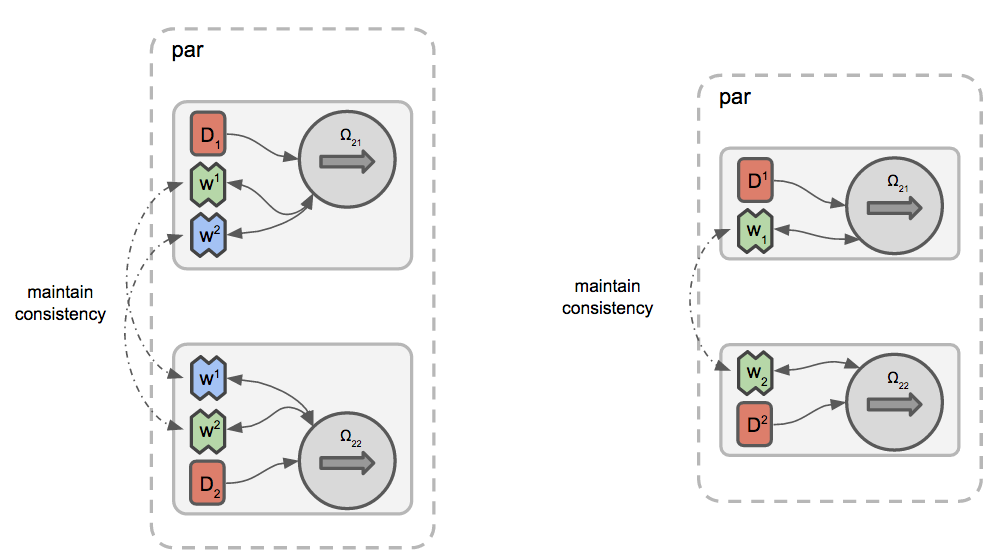
\includegraphics[width=0.9\textwidth]{img/par_repl_model.png}
\caption{Partitioned and Replicated State}
\label{fig:par_repl_model}
\end{figure}
As depicted in Figure \ref{fig:par_repl_model}, read-only states such as the input data $D$ are not subject to consistency management, whereas states that are altered by more than one unit in parallel must be kept consistent.
This stems from the fact that during the execution of a unit in parallel a non read-only state is in general subject to local and remote updates.
Depending on the partitioning the strategy to keep a state consistent varies slightly.
In case a state is partitioned across machines, there exists a main partition for each part of the state, containing the source of truth.
All units working in parallel on this part of the state, communicate the updates to the machine holding the main partition and also fetch the latest updates from this partition.
On the other hand, if a state is replicated there is no main partition holding the latest version of the state.
In this case each unit either has to broadcast all updates to all other parallel units or the units have to elect a unit that acts as the source of truth.
E.g. in case of the example depicted in Figure \ref{fig:ica_control_flow_dist}, unit $\Omega_{2i}$ updates its model $w_i$ locally based on some update procedure $\Delta$, according to (\ref{eqn:local_delta_upd}), but also receives the models $w_j, j \neq i$ of units $\Omega_{2j}, j \neq i$ as it is necessary to incorporate the progress of parallel instances in order to increase the algorithm throughput and mitigate slower convergence due to stale models.
The frequency at which the progress communication takes place is controlled by the consistency management based on the collected feedback.
As the second part of the consistency management must be present on each machine, the question arises which part on these machines is best suited to be responsible for controlling the consistency on a state level.

\section{State-centric vs. Computation-centric}
From an architectural perspective, two solutions can be considered for integrating the consistency management into each machine.
First, with state-centric consistency, as depicted in Figure \ref{fig:state_centric_consistency}, the consistency management is part of the state itself.
\begin{figure}[ht]
\centering
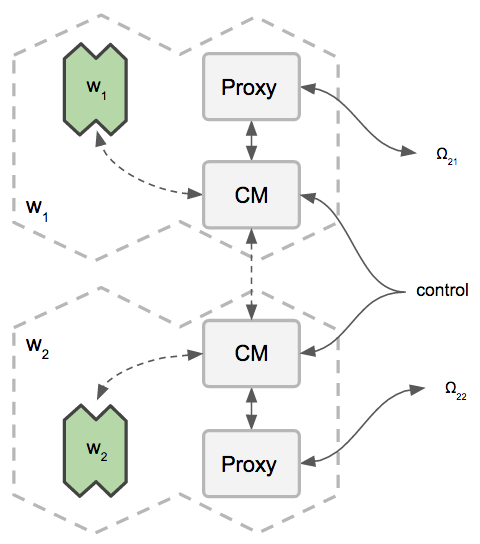
\includegraphics[width=0.5\textwidth]{img/state_centric_consist.png}
\caption{State-Centric Consistency Management}
\label{fig:state_centric_consistency}
\end{figure}
The consistency management and actual state are hidden behind a proxy, which mimics the interface of the state.
Each update is forwarded to the consistency management, which takes care of updating the local state as well as communicating updates to all other replicas or partitions depending on the partitioning.
The consistency management related parameters can be controlled by the driver.
This has the advantage that it offers a very convenient way to interact with a state because from a unit perspective a state behaves similar to a non-parallel version.
Furthermore, the design of a unit is considerably simplified as the computation is just a function that must be executed in parallel on multiple units and therefore very lightweight.
On the other hand, this approach requires a deep integration of consistency management logic into the state and therefore induces a tight coupling between logic and data.
This unnecessarily increases the dependency between data and framework and requires the developer to reimplement the logic in case the type of state changes.

Second, with computation-centric consistency, as can be seen in Figure \ref{fig:computation_centric_consistency}, the consistency management is part of the unit.
\begin{figure}[ht]
\centering
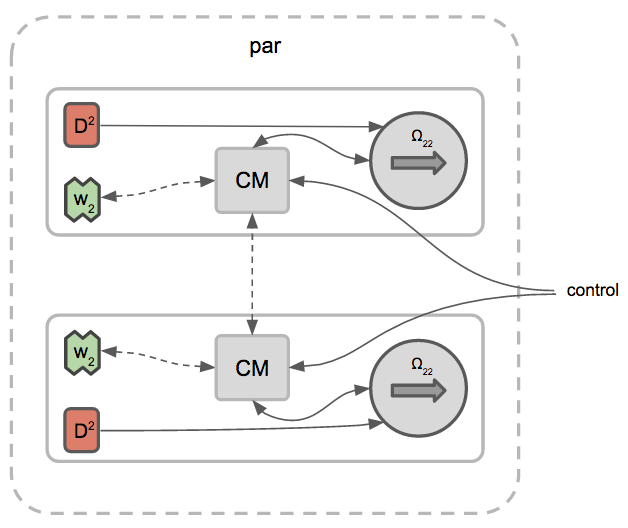
\includegraphics[width=0.5\textwidth]{img/computation_centric_consist.png}
\caption{Computation-Centric Consistency Management}
\label{fig:computation_centric_consistency}
\end{figure}
No coupling between state and framework exists, which makes it easier for a developer to reuse existing code.
Furthermore it provides a better abstraction due to the separation of logic and data and also a unit is already a part of the control-flow, responsible for executing the computational part.
Lastly, no proxy is required, which considerable simplifies the process of adding new types of state to the framework or reuse existing implementations such as matrix libraries.
In this architecture, the consistency management is periodically invoked to communicate with the driver in order to fetch new instructions and exchange progress with parallel units.

\section{Unit-internal Control-flow}
Considering both approaches, computation-centric consistency seems the best fit for the framework.
Therefore, in order to achieve the greatest flexibility and fine grained control over the consistency during algorithm execution, the consistency management is part of the unit itself.
Figure \ref{fig:unit_internal_flow} depicts the unit internal control-flow that is executed when the unit execution is triggered.
The control-flow contains the actual computation followed by a number of steps associated with consistency management.
\begin{figure}[ht]
\centering
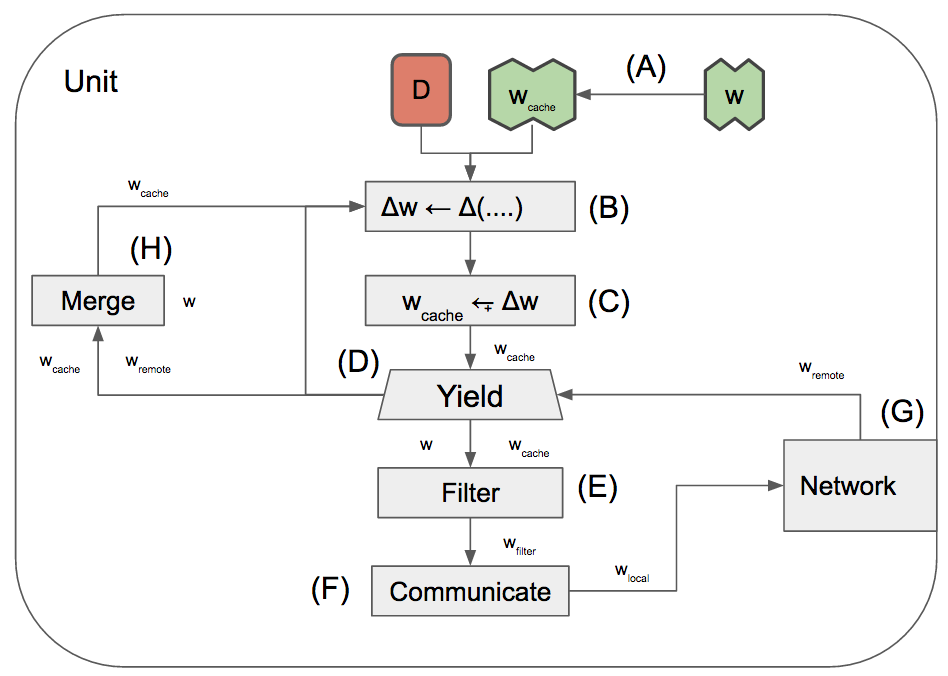
\includegraphics[width=0.9\textwidth]{img/unit_internal_flow.png}
\caption{Unit-Internal Control-flow}
\label{fig:unit_internal_flow}
\end{figure}
Previous to executing the computation enclosed in a unit, a cache is created for each state that is altered by said computation (A).
The reasoning behind this strategy is the fact that updates to the state are best communicated as relative change compared to a previous state (e.g. previous iteration), whereas the actual algorithm requires the absolute change.
In order to be able to compute a delta between two defined states, only the cache is altered and compared with the previous version before communicating updates.
After this initialization step the actual computation $\Delta(\ldots)$ is executed according to (\ref{eqn:delta_upd}), which results in a delta $\Delta w$ that can be used to update the state $w$.
Instead of applying the delta to actual state $w$, it is applied to the cache $w_{cache}$ only (C).
When running iterative-convergent algorithms this procedure of updating and caching is repeated multiple times according to the algorithm definition.
In order for the consistency management to gain a fine grained control over the update communication frequency during the execution, step (D) in the control-flow is a yield component similar to the primitive used in coroutines.
As with coroutines, the yield suspends the execution of the (update) computation in favor of executing other tasks.
In case of a unit with consistency management, the yield is triggered on request of the consistency management and at a frequency that is agreed on with the other replicas of the unit.
Upon a yield, the local progress is communicated to the other units $\Omega_{ij}$ in order to ensure a consistent state.
For this to happen, the actual state $w$ and the cached version $w_{cache}$ are used to compute $\Delta w = w_{cache} - w$, which is then forwarded to the filter stage (E) if configured.
The filter stage provides the developer with the ability to control which updates are actually forwarded to the communication stage (F) based on a defined criterion.
This is necessary for example when there is a bandwidth quota for each machine/unit and only a subset of the updates can be communicated.
All updates passing the filter stage are then forwarded to the communication stage and sent to the other units over the network (G).
Furthermore, if remote updates $w_{remote}$ have been received over the network, these are merged into the actual state $w$ together with the locally cached updates $w_{cache}$ (H).
A summary of merge strategies together with filter strategies is described in the following section.


\section{Strategies}
When executing an algorithm in parallel on a cluster of machines, often additional constraints are induced by the architecture.
For example, multiple independent tasks could be executed on the same machine and therefore a quota on resources like network bandwidth is enforced on a process level.
In such cases the consistency management needs additional means to identify the updates that are most important to the algorithm progress.
Filtering or prioritizing updates allows the consistency management to identify the most important updates that need to be communicated first without exceeding the network quota.

\subsection{Filter}
The simplest strategy for prioritizing updates is randomly choosing updated parameters of the state for communication until the network quota is exceeded.
Round-robin prioritization on the other hand repeatedly selects parameters following a fixed schedule.
A more data-driven approach takes the absolute magnitude of the change
\begin{equation}
\mid\Delta w\mid = \mid w - w_{cache} \mid
\label{eqn:absolute_magnitude}
\end{equation}
into account when deciding which parameters to communicate first.
Depending on the algorithm, the relative change in magnitude
\begin{equation}
\mid\frac{\Delta w}{a} \mid = \mid\frac{w - w_{cache}}{a} \mid
\label{eqn:relative_magnitude}
\end{equation}
might be a better prioritization strategy, where $a$ is the current value of the parameter.

\subsection{Merge}
In addition to prioritization, the merging strategy must be specified as well.
Merging refers to the process of combining local updates $w_{local}$, remote updates $w_{remote}$ and the current state $w$ to form an updated version of this particular state.
Merging in general can be described by
\begin{equation}
w_{i}^{t} = w_{i}^{t-1} + \gamma\sum_{k = 0}^{K}\Delta w_{k}
\label{eqn:state_merging}
\end{equation}
where $w_i^t$ is the updated state at time $t$, computed by updating the previous version of the state with a weighted sum of the remote states updates $\Delta w_k, k \neq i$ and the local updates $\Delta w_k, k = i$.
Depending on the partitioning of the state and the algorithm employed, the parameter $\gamma$ is commonly chosen to be either $\frac{1}{K}$ (averaging) or $1$ (adding).

%!TEX root = ./../thesis.tex

\chapter{Experiments}
\label{c:experiments}

\chapter{Conclusion}

%\include{chap1}
%\include{chap2}
\appendix
%\include{appa}
%\include{appb}
%% This defines the bibliography file (main.bib) and the bibliography style.
%% If you want to create a bibliography file by hand, change the contents of
%% this file to a `thebibliography' environment.  For more information 
%% see section 4.3 of the LaTeX manual.
\begin{singlespace}
\bibliography{thesis}
\bibliographystyle{plain}
\end{singlespace}

\end{document}

